\section{Technological Analysis}
% For each decision: requirement -> alternatives -> evidence -> trade-offs -> decision.
The analysis starts from five requirements derived from Section~I: (R1) each cone within a provisional tolerance of 15~cm of its planned position over tracks of 200~m or more; (R2) operation by one person with one Android phone; (R3) operation on a field without reliable mobile coverage; (R4) a twin that updates within about one second and accepts edits in both directions; and (R5) development effort compatible with one semester. Table~\ref{tab:decisions} summarises how the evidence of Section~II leads to each decision.

\begin{table*}[!t]
\caption{Approaches for aligning the track plan to the real ground}
\label{tab:alignment}
\centering
\footnotesize
\setlength{\tabcolsep}{4pt}
\renewcommand{\arraystretch}{1.15}
\begin{tabular}{|L{0.15\textwidth}|L{0.17\textwidth}|L{0.18\textwidth}|L{0.09\textwidth}|L{0.13\textwidth}|L{0.08\textwidth}|L{0.07\textwidth}|}
\hline
\textbf{Approach} & \textbf{Reported accuracy} & \textbf{Range and drift} & \textbf{Cost} & \textbf{Setup effort} & \textbf{People} & \textbf{Sources} \\ \hline
Tape and trigonometry (baseline) & Not reported; depends on the operator & No drift; errors accumulate per measurement & Very low & High & Two or more & Team practice \\ \hline
Single start marker & About 5~cm near the marker, worse further away & Heading error grows with distance; drift up to 17~m per 120~m & Low & Low & One & \cite{chalhoub2019}, \cite{feigl2020} \\ \hline
Two-point alignment + re-alignment markers & Two markers reduce angular error~\cite{nunes2023}; not tested on phones over a track & Drift limited to the distance between markers & Low & Medium (markers placed once per site) & One & \cite{nunes2023}, \cite{chalhoub2019} \\ \hline
Geospatial API (visual positioning) & No published centimetre-level figures & Needs Street View coverage & Free & Low & One & \cite{arcoregeo}, \cite{skabek2026} \\ \hline
Smartphone RTK GNSS & 1.1--4~cm RMS in open sky & No drift; needs sky view and corrections & Medium & Medium & One & \cite{jiang2023} \\ \hline
\end{tabular}
\end{table*}

\begin{figure*}[!t]
\centering
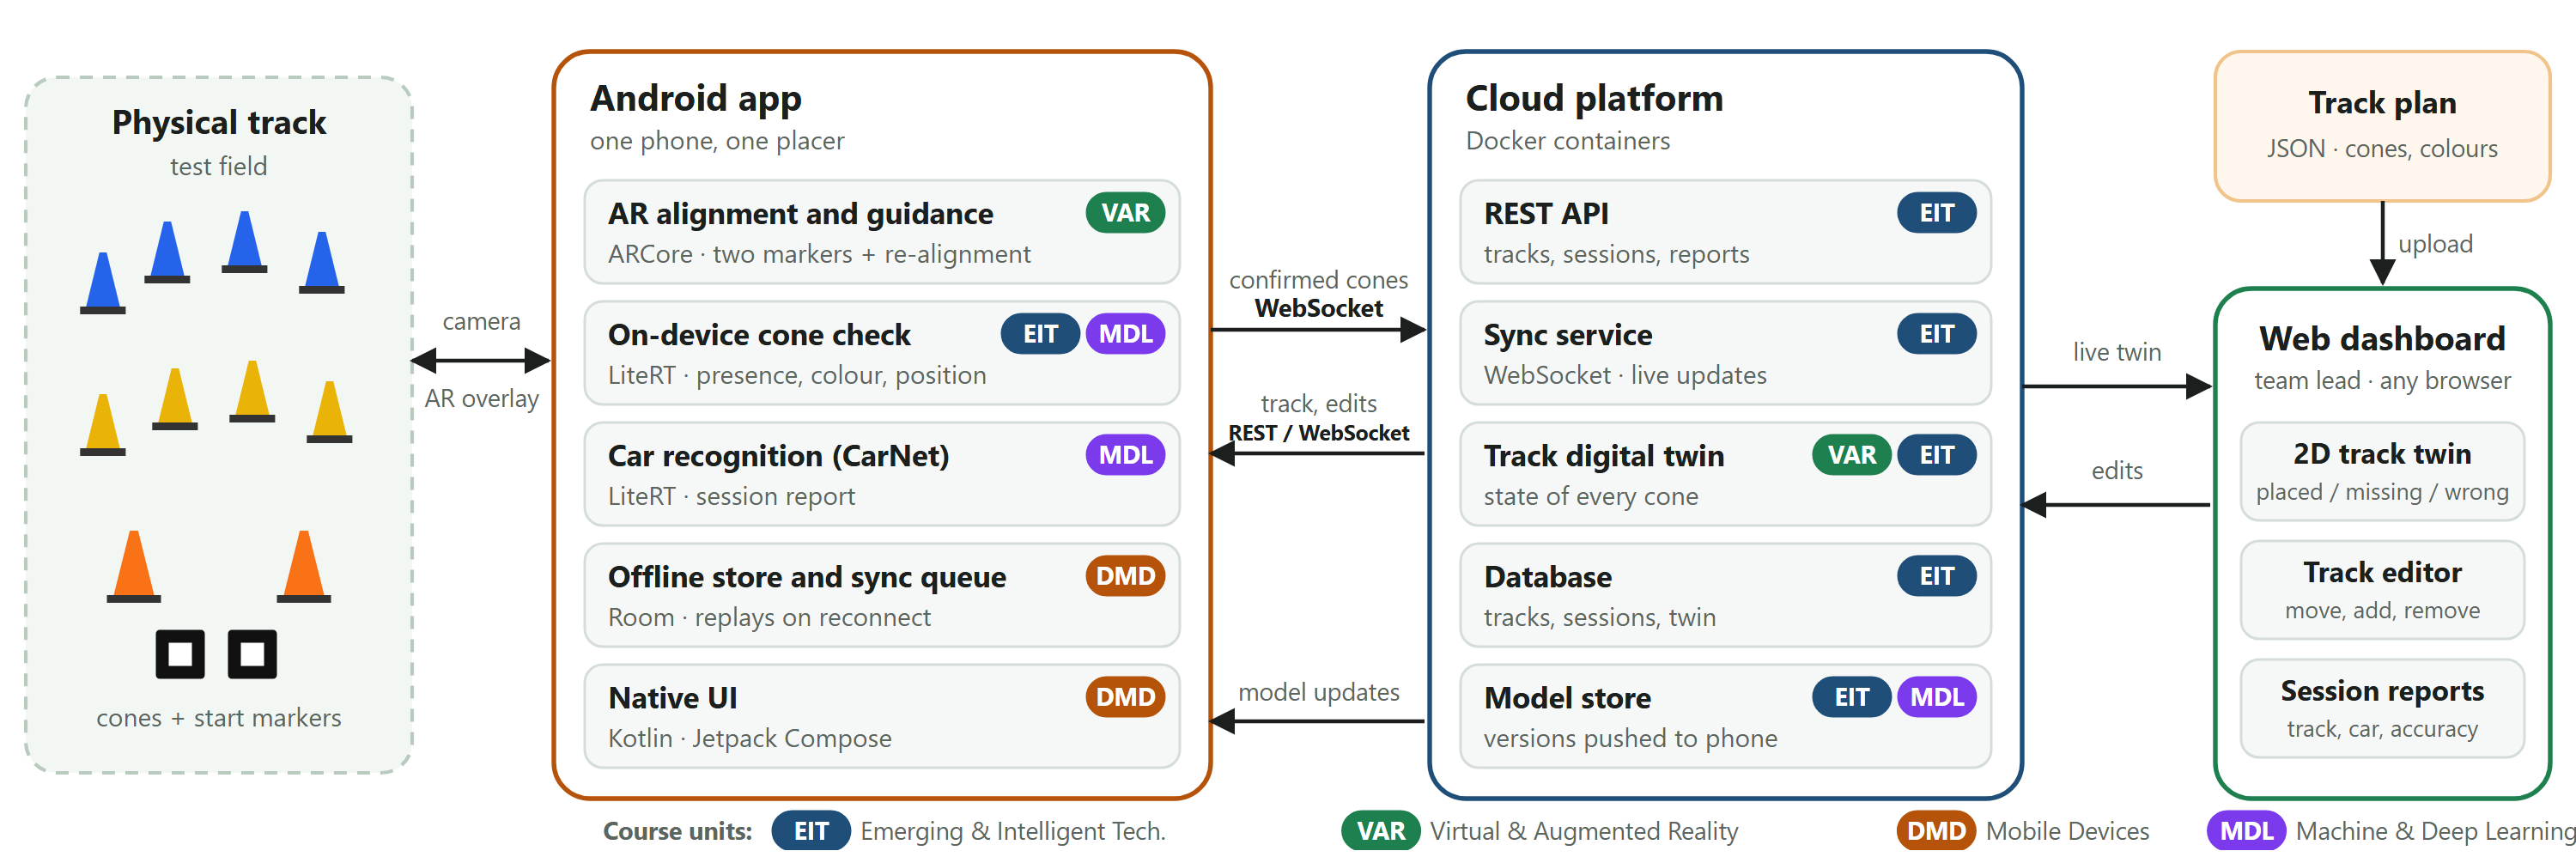
\includegraphics[width=\textwidth]{assets/trackseed_architecture.png}
\caption{Conceptual architecture of TrackSeed. The phone guides and verifies the placement on the physical track and sends each confirmed cone to the cloud over WebSocket; the cloud keeps the track twin, which the dashboard displays live, and returns track edits and model updates to the phone. Tags show the course unit responsible for each part.}
\label{fig:architecture}
\end{figure*}

\subsection{Aligning the track plan to the ground}
Alignment is driven by R1 and R2, against which Table~\ref{tab:alignment} compares the options. The tape method fails R2, since it needs two or more people. A single marker at the start line is the simplest option, but it fixes the heading of the whole plan from a marker less than a metre wide: a heading error of only $1^\circ$ moves a cone 200~m away by about 3.5~m, and visual-inertial drift adds to this as the user walks~\cite{feigl2020}. Aligning on two markers placed far apart fixes position and heading together, and re-aligning at further markers along the track limits the drift to the distance between markers. Both steps are supported by the literature: Nunes et al.\ found that two markers significantly reduce the angular error of one~\cite{nunes2023}, and error is smallest near the reference~\cite{chalhoub2019}. The Geospatial API is rejected as the main method because no evidence shows it reaches the required accuracy~\cite{arcoregeo}. RTK GNSS reaches centimetre accuracy without drift~\cite{jiang2023}, but needs a correction service and suitable hardware; it is kept as an optional extension, to be added only if field tests show that marker alignment cannot meet R1. TrackSeed therefore adopts two-point marker alignment with re-alignment markers. Two decisions remain open: the spacing between markers, to be set from field tests, and how the markers are positioned, which only needs to be done once per site with the team's usual method or an RTK receiver.

\subsection{Mobile AR platform}
The platform is driven by R2, which fixes the device to one Android phone, and by R1, through the quality of tracking. Native Android with ARCore, Unity with AR Foundation and native iOS with ARKit were considered. Native Android in Kotlin gives direct access to the ARCore session and its camera frames, which the on-device cone check needs. Unity would add cross-platform reach that R2 does not require, at the cost of an extra runtime layer between the camera and the model. For R1, tracking quality does not separate the platforms: Scargill et al.\ found neither uniformly better, and ARCore drifted less when the user walked away and returned~\cite{scargill2021}, the movement most similar to walking between cones. The compromise is that the app runs only on ARCore-supported Android phones; other users reach the twin through the web dashboard.

\subsection{Platform and real-time communication}
Communication is driven by R3: each confirmed cone and each edit must reach the other side within about one second. Table~\ref{tab:comms} compares the options. REST polling would make R3 depend on the polling interval. TrackSeed sends one small message per confirmed cone, and the dashboard runs in a browser; in this setting, WebSocket's lower latency~\cite{ajayi2023} and native browser support outweigh MQTT's higher throughput and lower resource use, which matter for many constrained devices rather than one phone. A managed real-time database would provide offline synchronisation out of the box~\cite{firebaseoffline}, but it ties the platform to one provider and gives less control over the twin's data model. TrackSeed therefore uses WebSocket for live updates and REST for uploading and downloading tracks and reports. So that no confirmation is lost if the connection drops, the phone also stores every confirmed cone locally and resends the queued messages when the connection returns, the same pattern a managed database applies internally. The services run in Docker containers, and tracks use an open JSON schema so that plans from other FS tools can be imported.

\begin{table}[!t]
\caption{Real-time communication options}
\label{tab:comms}
\centering
\footnotesize
\setlength{\tabcolsep}{3pt}
\renewcommand{\arraystretch}{1.12}
\begin{tabular}{|L{0.16\columnwidth}|L{0.19\columnwidth}|L{0.19\columnwidth}|L{0.17\columnwidth}|L{0.15\columnwidth}|}
\hline
\textbf{Option} & \textbf{Latency} & \textbf{Offline support} & \textbf{Scale} & \textbf{Effort} \\ \hline
REST polling & Limited by the polling interval & Client must queue writes & Many redundant requests & Low \\ \hline
WebSocket & Lower than MQTT~\cite{ajayi2023} & Client must queue writes & One connection per client & Medium; native in browsers \\ \hline
MQTT & Slightly higher~\cite{ajayi2023} & Session state kept by the protocol~\cite{mqtt5} & Higher throughput, fewer resources~\cite{ajayi2023} & Medium; needs a broker \\ \hline
Managed real-time DB & Not compared & Local cache and queued writes~\cite{firebaseoffline} & Managed by provider & Low; vendor lock-in \\ \hline
\end{tabular}
\end{table}

\subsection{Digital twin and on-device intelligence}
The twin stores, for every cone, its planned position and colour and a state: planned, placed, verified, wrong colour or missing, with the measured offset. Because cones lie on a plane, a 2D top-down map is enough for the dashboard; a 3D view is optional. Edits made on the dashboard go through the sync service to the phone and change the guidance; the placer then moves the cone, so the loop back to the physical track goes through a person. The cone check serves R1, since it measures the offset of every placed cone, and where it runs affects R3: on the phone, only a small confirmation message has to travel over the network, instead of camera frames~\cite{chen2019}. Following Section~II-D, the check therefore runs on the phone with a compressed model in LiteRT, while the cloud stores training data and pushes new model versions, which also provides remote configuration. A second on-device model, developed in the Machine and Deep Learning course, recognises the team car at the end of a session for the report.

\begin{table}[!t]
\caption{From research findings to design decisions}
\label{tab:decisions}
\centering
\footnotesize
\setlength{\tabcolsep}{3pt}
\renewcommand{\arraystretch}{1.12}
\begin{tabular}{|L{0.27\columnwidth}|L{0.27\columnwidth}|L{0.27\columnwidth}|L{0.08\columnwidth}|}
\hline
\textbf{Evidence} & \textbf{Implication} & \textbf{Decision} & \textbf{Req.} \\ \hline
AR accuracy degrades with distance from the marker~\cite{chalhoub2019} & One marker cannot keep a 200~m track within tolerance & Two-point alignment at the start & R1, R2 \\ \hline
Tracking error grows with distance walked~\cite{feigl2020} & Phone tracking alone cannot hold a full lap & Re-alignment markers; RTK as an option~\cite{jiang2023} & R1 \\ \hline
Neither ARCore nor ARKit is uniformly better~\cite{scargill2021} & Tracking quality does not decide the platform & Native Android, the single device of R2 & R1, R2 \\ \hline
WebSocket has lower latency, MQTT higher throughput~\cite{ajayi2023} & One small message per cone; the client is a browser & WebSocket, with a resend queue on the phone & R3 \\ \hline
On-device inference avoids network latency and privacy costs~\cite{chen2019} & Only a small message per cone needs the network & Cone check on the phone; models updated remotely & R1, R3 \\ \hline
\end{tabular}
\end{table}
